\documentclass{article}

\usepackage{tikz}
\usepackage{amsmath}
\usepackage{amssymb}
\usepackage{bm}
\usepackage{algpseudocode}
\usepackage{algorithm}
\usetikzlibrary{bayesnet}

\DeclareMathOperator*{\argmax}{arg\,max}

\title{EM Algorithm for Labeled IRL}
\author{James MacGlashan}
\date{}
\begin{document}

\maketitle

\section{Introduction}
In this document, I explored the EM algorithm approach to solving our labeled IRL problem. As a review, I first include the description of our model that we've previously defined and then provide the EM algorithm approach.

\section{Probability Model}
The motivation for this model is that we consider the the final label ($L$) that a user gives a trajectory of size $N$ to be some random function of what they thought about each of the action selections ($A$) exhibited in the trajectory. However these step-wise evaluations ($X$) are unobserved in the data.
\begin{figure}
\centering
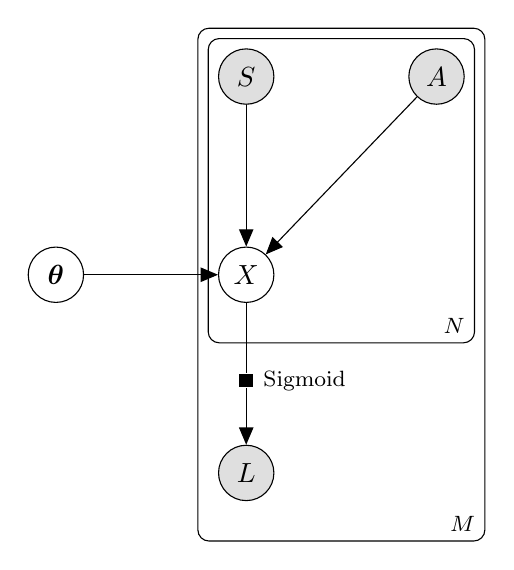
\begin{tikzpicture}[x=1.7cm,y=1.8cm]
   \node[latent]                   (R)      {$\bm{\theta}$} ; %
   \node[latent, right=of R]                   (X)      {$X$} ; %
   \node[obs, below=of X]                      (L)      {$L$} ; %
   \node[obs, above=of X]          (S)      {$S$} ; %
   \node[obs, right=of S]          (A)      {$A$} ; %
   
   \factor[above=of L]{L-f}{right:Sigmoid}{}{} ;

  \edge {S}{X} ;
  \edge {A}{X} ;
  \edge {R}{X} ;
  \factoredge {X}{L-f}{L} ;

   \plate {traj}{
   		(S) (A) (X)
   } {$N$} ;%

   \plate {data}{
   		(traj)(L-f)(L)
   } {$M$} ;

\end{tikzpicture}
\caption{Plate Diagram of our Probability Model}
\label{fig:gm}
\end{figure}

We model the probability that an action is evaluated as good or not as proportional to its selection probability according a softmax policy computed for the reward function with parameters $\bm{\theta}$. Specifically:
\begin{align}
\Pr(x_i = +1 | s, a, \theta) &= \pi(s, a | \bm{\theta}) \\
\Pr(x_i = -1 | s, a, \theta) &= 1 - \pi(s, a | \bm{\theta}),
\end{align}
where $\pi(s, a | \bm{\theta})$ is the softmax policy over Q-values computed for the reward function parameterized by $\bm{\theta}$:
\begin{equation}
\pi(s, a | \bm{\theta}) = \frac{e^{\beta Q(s,a | \bm{\theta})}}{\sum_{a'}e^{\beta Q(s,a' | \bm{\theta})}},
\end{equation}
$\beta$ is a selectable parameter, and $Q(s,a|\bm{\theta})$ is the Q-value computed for the reward function parameterized by $\bm{\theta}$.


For the probability distribution of $L$, given the sequence of $N$ step-wise labels, we would like a distribution that has the property that as more step-wise labels are positive, the probability of a positive trajectory label increases (and vice versa). Although there are many possible distributions that satisfy this property, for concreteness, we choose the sigmoid function. That is,
\begin{align}
\Pr(L = +1 | X_1, ..., X_n) &= \frac{1}{1 + e^{-\phi \sum_i^N X_i}} \\
\Pr(L = -1 | X_1, ... ,X_n) &= 1 - \Pr(L = +1 | X_1, ..., X_n),
\end{align}
where $\phi$ is a selectable parameter that tunes how quickly of a majority of step-wise labels increases/decreases the probability of trajectory assignment. For example, when $\phi = 0$, trajectory labels are assigned uniformly randomly independently of step-wise labels. As $\phi \rightarrow \infty$, the sigmoid converges to a step function in which a trajectory containing even one more positive step-wise label than negative step-wise labels will deterministically cause a positive trajectory label (and vice versa).

\section{EM Algorithm}
The problem with estimating the $\bm{\theta}$ parameters of our reward function is that we have a latent variable vector $X$ (or rather, some of the elements of the $X$ vector are latent, and some may be observed), which prevents us from easily computing the likelihood of the model and maximizing parameters for it. The EM approach to solving this problem is to first choose values for $\bm{\theta}$; then choose a new $\bm{\theta}$ that maximizes the expected value of the log likelihood function where the distribution of the expectation is the probability distribution of latent variables (the $X$s in our case) given the observations available and previous $\bm{\theta}$ choice; and then repeating this process. The maximization process can be performed using gradient ascent. 

To formalize this process for our problem, first note that the likelihood our parameters (and state-action sequence) given an $\bm{x}$ vector and label $l$ is
\begin{align}
\mathcal{L}(\bm{s}, \bm{a}, \bm{\theta} | l, \bm{x}) = \Pr(l | \bm{x}) \prod_i \Pr(x_i | s_i, a_i, \bm{\theta})
\end{align}
and the log likelihood is
\begin{align}
\log\mathcal{L}(\bm{s}, \bm{a}, \bm{\theta} | l, \bm{x}) = \log \Pr(l | \bm{x}) + \sum_i \log \Pr(x_i | s_i, a_i, \bm{\theta}).
\end{align}
Additionally, the gradient of the log likelihood is,
\begin{align}
\nabla_{\bm{\theta}} \log\mathcal{L}(\bm{s}, \bm{a}, \bm{\theta} | l, \bm{x}) = \sum_i  \frac{\nabla_{\bm{\theta}} \Pr(x_i | s_i, a_i, \bm{\theta})}{\Pr(x_i | s_i, a_i, \bm{\theta})}.
\end{align}

To simplify the EM algorithm description, I will introduce the notation $\bm{x}_k$ to indicate the subset of observed elements in an $\bm{x}$ vector, and $\bm{x}_u$ to represent a possible assignment to the subset of the unobserved values of an $\bm{x}$ vector. Using this notation, the expected value of the log likelihood under some candidate parameter $\bm{\theta}'$ for missing $X$ elements distributed according to $\bm{\theta}$ is
\begin{align*}
E_{\bm{x}_u \sim \Pr(\bm{x}_u | l, \bm{x}_k, \bm{s}, \bm{a}, \bm{\theta})} & \left[ \log\mathcal{L}(\bm{s}, \bm{a}, \bm{\theta}' | l, \bm{x}) \right] \\ &= \sum_{\bm{x}_u} \Pr(\bm{x}_u | l, \bm{x}_k, \bm{s}, \bm{a}, \bm{\theta}) \log\mathcal{L}(\bm{s}, \bm{a}, \bm{\theta}' | l, \bm{x})
\end{align*}


Given that, the corresponding EM algorithm operating on a single trajectory is as follows (it is generalized to many trajectories by simply summing over each trajectory).
\begin{algorithm}
\caption{Labeled-IRL EM Algorithm}
\begin{algorithmic}
\Require{initial $\bm{\theta}_0$, and data $\bm{s}$, $\bm{a}$, $\bm{x}_k$, $l$}
\For{$t=0$ to $K$}
\State $\bm{\theta}_{t+1} \gets \argmax_{\bm{\theta'}} \sum_{\bm{x}_u} \Pr(\bm{x}_u | l, \bm{x}_k, \bm{s}, \bm{a}, \bm{\theta}_t) \log\mathcal{L}(\bm{\theta'}, \bm{s}, \bm{a} \mid l, \bm{x}_k, \bm{x}_u)$
\EndFor
\end{algorithmic}
\end{algorithm}

To compute the expected value, we need to enumerate each of the possible assignments to the unknown $\bm{x}$ elements and compute the probability of them given the observed data and model parameters $\bm{\theta}$.  This probability is computed as
\begin{align*}
\Pr(\bm{x}_u | l, \bm{x}_k, \bm{s}, \bm{a}, \bm{\theta}) &= \frac{\Pr(l | \bm{x}_k, \bm{x}_u) \Pr(\bm{x}_u | \bm{s}, \bm{a}, \bm{\theta}) \Pr(\bm{x}_k | \bm{s}, \bm{a}, \bm{\theta}) \Pr(\bm{s}, \bm{a}, \bm{\theta})}{\Pr(l | \bm{x}_k, \bm{s}, \bm{a}, \bm{\theta}) \Pr(\bm{x}_k | \bm{s}, \bm{a}, \bm{\theta}) \Pr(\bm{s}, \bm{a}, \bm{\theta})} \\
 &= \frac{\Pr(l | \bm{x}_k, \bm{x}_u) \Pr(\bm{x}_u | \bm{s}, \bm{a}, \bm{\theta}) }{\Pr(l | \bm{x}_k, \bm{s}, \bm{a}, \bm{\theta})} \\
 &= \frac{\Pr(l | \bm{x}_k, \bm{x}_u) \prod_i \Pr(\bm{x}_{u,i} | s_i, a_i, \bm{\theta}) }{\Pr(l | \bm{x}_k, \bm{s}, \bm{a}, \bm{\theta})}. 
\end{align*}
A straight forward computation of $\Pr(l | \bm{x}_k, \bm{s}, \bm{a}, \bm{\theta})$ requires marginalizing over all possible assignment to the unknown $X$ elements; however, it can be computed efficiently using dynamic programming because the probability of a label is a sigmoid function that operates on the sum of the $x$ elements. I will not cover the dynamic programming computation of it here.

Unfortunately, even with an efficient means to compute $\Pr(l | \bm{x}_k, \bm{s}, \bm{a}, \bm{\theta})$, when the number of unknown $X$ variables is large, the number of $\bm{x}_u$ assignments enumerated in the expectation's outer sum grows exponentially, and the product series over each of unknown element probabilities in the above equation ($\prod_i \Pr(\bm{x}_{u,i} | s_i, a_i, \bm{\theta})$) can have underflow issues. A resolution to this problem is to estimate the expectation with sampling. Monte Carlo sampling is unfortunately intractable because it is not easy to sample from $\Pr(\bm{x}_u | l, \bm{x}_k, \bm{s}, \bm{a}, \bm{\theta})$; moreover, it would not address the underflow issue in the product series. However, it is easy to sample from $\Pr(\bm{x}_u | \bm{s}, \bm{a}, \bm{\theta})$ (removing the conditioning on the label), which we can use in importance sampling. With importance sampling, we can replace the expectation computation with the sample-estimate
\begin{equation}
\frac{1}{C} \sum_j^C \frac{\Pr(\bm{x}_u^j | l, \bm{x}_k, \bm{s}, \bm{a}, \bm{\theta})}{\Pr(\bm{x}_u^j | \bm{s}, \bm{a}, \bm{\theta})} \log\mathcal{L}(l, \bm{x}_k, \bm{x}_u^j | \bm{s}, \bm{a}, \bm{\theta}).
\end{equation}
where $\bm{x}_u^j$ is sample from the distribution $\Pr(\bm{x}_u | \bm{s}, \bm{a}, \bm{\theta})$.

Note that this simplifies a bit further too:
\begin{align*}
\frac{\Pr(\bm{x}_u^j | l, \bm{x}_k, \bm{s}, \bm{a}, \bm{\theta})}{\Pr(\bm{x}_u^j | \bm{s}, \bm{a}, \bm{\theta})} &= \frac{\Pr(l | \bm{x}_k, \bm{x}_u) \Pr(\bm{x}_u^j | \bm{s}, \bm{a}, \bm{\theta}) }{\Pr(l | \bm{x}_k, \bm{s}, \bm{a}, \bm{\theta})} \frac{1}{\Pr(\bm{x}_u^j | \bm{s}, \bm{a}, \bm{\theta})} \\
&= \frac{\Pr(l | \bm{x}_k, \bm{x}_u)}{\Pr(l | \bm{x}_k, \bm{s}, \bm{a}, \bm{\theta})}
\end{align*}
Consequently, we have removed the product series from the expectation weight, thereby avoiding underflow issues. Also, as noted previously, the $\Pr(l | \bm{x}_k, \bm{s}, \bm{a}, \bm{\theta})$ term can be computed efficiently with dynamic programming.

Now we can write a tractable EM algorithm where we can compute the maximization using gradient ascent.

\begin{algorithm}
\caption{Labeled-IRL Approximate EM Gradient Ascent Algorithm}
\begin{algorithmic}
\Require{initial $\bm{\theta}_0$; data $\bm{s}$, $\bm{a}$, $\bm{x}_k$, $l$; and learning rate $\alpha$}
\For{$t=0$ to $K$}
\State draw $j =1$ to $C$ samples of $\bm{x}_u^j \sim \Pr(\bm{x}_u | \bm{s}, \bm{a}, \bm{\theta}_t)$ 
\For{$j=1$ to $C$}
\State $w_j \gets \frac{\Pr(l | \bm{x}_k, \bm{x}_u)}{\Pr(l | \bm{x}_k, \bm{s}, \bm{a}, \bm{\theta}_t)}$ \Comment{Expectation step}
\EndFor
\State $\bm{\theta}' \gets \bm{\theta}_t$
\For{1 to $M$} \Comment{Gradient ascent maximization loop}
\State $\bm{\theta}' \gets \bm{\theta}' + \alpha \frac{1}{C} \sum_j^C w_j \sum_{x_i \in \bm{x}_k \cup \bm{x}_u^j} \frac{\nabla_{\bm{\theta}'} \Pr(x_i | s_i, a_i, \bm{\theta}')}{\Pr(x_i | s_i, a_i, \bm{\theta}')} $
\EndFor
\State $\bm{\theta}_{t+1} \gets \bm{\theta}'$
\EndFor
\end{algorithmic}
\end{algorithm}

\section{DP Algorithm For Label Probability}
One of the terms that must be computed for the EM algorithm weight is $\Pr(l \mid \bm{x}_k, \bm{s}, \bm{a}, \bm{\theta})$. A straightforward computation of this value would involve marginalizing over $\bm{x}_u$, which grows exponentially large as the number of unknown feedbacks increases. However, by exploiting the fact that $\Pr(l | \bm{x}_k, \bm{x}_u, \bm{s}, \bm{a}, \bm{\theta})$ is a function of the sum of the feedback values, the marginalization can be reduced to a summation that iterates over a number of values that is a linear function of the number of unobserved feedbacks. To demonstrate, first note that $\Pr(l \mid \bm{x}, \bm{s}, \bm{a}, \bm{\theta})$, where all feedback values are known, is defined as
\begin{equation}
\Pr(l \mid \bm{x}, \bm{s}, \bm{a}, \bm{\theta}) = S\left(\sum_{x \in \bm{x}} x \right),
\end{equation} 
where $S$ is the sigmoid function. Therefore, $\Pr(l \mid \bm{x}_k, \bm{s}, \bm{a}, \bm{\theta})$, where some of the feedbacks are unobserved, can expressed by marginalizing over the possible {\em sums} of the unknown feedbacks, rather than marginalizing over all possible feedback assignments:
\begin{equation}
\Pr(l \mid \bm{x}_k, \bm{s}, \bm{a}, \bm{\theta}) = \sum_{\tau = -|\bm{x}_u|}^{|\bm{x}_u|} S\left(\tau + \sum_{x \in \bm{x}_k} x\right) \Pr(\tau \mid \bm{s}_u, \bm{a}_u, \bm{\theta}),
\end{equation}
where $\Pr(\tau \mid \bm{s}_u, \bm{a}_u, \bm{\theta})$ is the probability that the unknown feedbacks will sum to $\tau$, given the states and actions for the unknown feedbacks, and the model parameters $\bm{\theta}$.

Computing this simpler marginal distribution requires computing $\Pr(\tau \mid \bm{s}_u, \bm{a}_u, \bm{\theta})$: the probability distribution of the sum of possible feedback values. Fortunately, this probability can expressed recursively and computed efficiently with a dynamic programming algorithm. 

To describe this recursive relationship, note that if we knew the probability distribution of the sum of feedback values for all unknown feedbacks except the last of them, then we could compute the probability that {\em all} of the feedbacks would some to some value $\tau$ as the probability that the remaining feedbacks sum to $\tau - 1$ and the last feedback is a $+1$ {\em or} the remaining feedbacks sum to $\tau + 1$ and the last feedback is a $-1$. That is,
\begin{align}
\Pr(\tau_n = \tau \mid \bm{s}_n, \bm{a}_n, \bm{\theta}) =& \Pr(x_n = +1 \mid s_n, a_n) \Pr(\tau_{n-1} = \tau_n - 1 \mid \bm{s}_{n-1}, \bm{a}_{n-1}, \bm{\theta}) \nonumber \\
& + \Pr(x_n = -1 \mid s_n, a_n) \Pr(\tau_{n-1} = \tau_n + 1 \mid \bm{s}_{n-1}, \bm{a}_{n-1}, \bm{\theta}), 
\end{align}
where $n$ is the number unobserved feedbacks, $\tau_i$ is the random variable specifying the sum of the first $i$ unobserved feedbacks; $s_i$ and $a_i$ represents the $i$th state and action that are associated with unobserved feedback $x_i$; $\bm{s}_i$, $\bm{a}_i$ represents the set of the first $i$ state and actions associated with the unobserved feedbacks; and finally, where the probability of the first unobserved feedback summing to $\tau$ is defined as the probability that the first feedback takes that value:
\begin{equation}
\Pr(\tau_1 = \tau \mid \bm{s}_n, \bm{a}_n, \bm{\theta}) = \begin{cases}
\Pr(x_n = +1 \mid s_n, a_n) & \mbox{if } \tau_1 = 1 \\
\Pr(x_n = -1 \mid s_n, a_n) & \mbox{if } \tau_1 = -1 \\
0 & \mbox{otherwise}
\end{cases}.
\end{equation}
We can compute this recursive probability distribution using dynamic programming in which we build a $2n+1 \times n$ matrix, where cell $i,j$ specifies the value for $\Pr(\tau_j = i \mid \bm{s}_j, \bm{a}_j, \bm{\theta})$. The values for the matrix are then filled out column by column, from $j=1$ to $n$. Consequently, using this DP algorithm, we can compute the $\Pr(l \mid \bm{x}_k, \bm{s}, \bm{a}, \bm{\theta})$ term required for our EM weight in only $O(|\bm{x_u}|^2)$ time, rather than $O(2^{|\bm{x_u}|})$.

\section{Other Importance Sampling Distributions}
One of the potential problems with the importance sampling distributions being drawn from the policy under the theta values that is as the agent optimizes for theta, it will produce more detemrinistic action selection, leading to progressively more biased samples that may not adequately cover the space. Indeed, initial experiments with the current distribution show that in some cases, the log likelihood starts getting worse, whereas when using the full marginalization, it consistently improves.

To comabt this issue, we should explore other sampling distributions that better span the space. One potential issue is that with a different sampling distribution, we must include the product series of the individual feedback probabilities, which could produce underflow. However, if we simply choose a slightly nosier sampling feedback distribution than the feedback distribution under the current parameters, then we might avoid underflow problems.

That is, let a vector for unknown feedbacks $\bm{x}_u$ be drawn from some sampling distribution $f$ that indepdently draws feedbacks as a function of each state-action pair and the current parameters $\theta$:
\begin{equation}
f(\bm{x}_u \mid \bm{s}, \bm{a}, \bm{\theta}) = \prod_i f_i(x_{u,i} \mid s_i, a_i, \bm{\theta}).
\end{equation}
Then using $f$ as the importance sampling distribution, we have the following importance sampling weights for each sample $x_u^j$:
\begin{align}
w_j &= \frac{\Pr(l | \bm{x}_k, \bm{x}_u^j) \Pr(\bm{x}_u^j | \bm{s}, \bm{a}, \bm{\theta}) }{\Pr(l | \bm{x}_k, \bm{s}, \bm{a}, \bm{\theta})} \frac{1}{f(\bm{x}_u^j \mid \bm{s}, \bm{a}, \bm{\theta})} \nonumber \\
&= \frac{\Pr(l | \bm{x}_k, \bm{x}_u^j) \prod_i \Pr(x_{u,i}^j | s_i, a_i, \bm{\theta}) }{\Pr(l | \bm{x}_k, \bm{s}, \bm{a}, \bm{\theta})} \frac{1}{\prod_i f_i(x_{u,i}^j \mid s_i, a_i, \bm{\theta})} \nonumber \\
&=\frac{\Pr(l | \bm{x}_k, \bm{x}_u^j)}{\Pr(l | \bm{x}_k, \bm{s}, \bm{a}, \bm{\theta})} \prod_i \frac{\Pr(x_{u,i}^j | s_i, a_i, \bm{\theta})}{f_i(x_{u,i}^j \mid s_i, a_i, \bm{\theta})}
\end{align}
Therefore, as long as $\frac{\Pr(x_{u,i}^j | s_i, a_i, \bm{\theta})}{f_i(x_{u,i}^j \mid s_i, a_i, \bm{\theta})}$ is reasonably near 1, there shouldn't be underflow issues. This condition may be held if the single feedback distribution $f_i$, is also based on a softmax policy distribution of the current weights theta, but is more uniform (e.g., a small $\beta$ value.) That is,
\begin{equation}
f_i(x_i \mid s_i, a_i, \bm{\theta}) = \begin{cases}
\frac{e^{\hat{\beta} Q(s,a | \bm{\theta})}}{\sum_{a'}e^{\hat{\beta} Q(s,a' | \bm{\theta})}} & \mbox{if } x_i = 1 \\
1 - \frac{e^{\hat{\beta} Q(s,a | \bm{\theta})}}{\sum_{a'}e^{\hat{\beta} Q(s,a' | \bm{\theta})}} & \mbox{if } x_i = -1
\end{cases},
\end{equation}
where $\hat{\beta} < \beta$ and $\beta$ is the normal softmax policy parameter used by our probability model (Equation 3), such that $f_i$ is a more nosiy, uniform response.


\end{document}